% =============================================================================
% Chapter 5: Token Embeddings
% =============================================================================
\chapter{Token Embeddings}
\label{ch:token-embeddings}

\begin{objectives}
    \item Understand how discrete tokens become continuous vectors
    \item Learn about embedding tables and lookup operations
    \item Grasp the concept of embedding dimensions
    \item Understand weight tying between input and output embeddings
\end{objectives}

% -----------------------------------------------------------------------------
\section{From Tokens to Vectors}
% -----------------------------------------------------------------------------

In the previous chapters, we converted text to sequences of integers (token IDs). But neural networks work best with continuous values, not discrete IDs. How do we bridge this gap?

The answer is \textbf{embeddings}---learned mappings from discrete tokens to continuous vectors.

\begin{definition}[title=Token Embedding]
A \textbf{token embedding} is a dense, learned vector representation of a token. Each token ID maps to a unique vector of dimension $d_{\text{model}}$.
\end{definition}

\subsection{Why Not One-Hot Encoding?}

You might think of representing token ID 42 as a vector with 1 at position 42 and 0 everywhere else. This is called \textbf{one-hot encoding}:

\begin{lstlisting}[style=python]
vocab_size = 16384
token_id = 42

# One-hot: sparse vector with single 1
one_hot = [0, 0, ..., 1, ..., 0, 0]  # 16384-dimensional!
\end{lstlisting}

Problems with one-hot encoding:
\begin{itemize}
    \item \textbf{High dimensionality}: Vector size equals vocabulary (16,384 dimensions)
    \item \textbf{No semantic similarity}: ``cat'' and ``kitten'' are equally distant as ``cat'' and ``airplane''
    \item \textbf{Sparse}: Wastes computation on zeros
\end{itemize}

\subsection{Learned Embeddings}

Instead, we learn a \textbf{dense} representation:

\begin{lstlisting}[style=python]
d_model = 384  # Embedding dimension

# Learned embedding: dense vector
embedding = [0.23, -0.87, 0.12, ..., 0.45]  # 384-dimensional
\end{lstlisting}

Benefits:
\begin{itemize}
    \item \textbf{Low dimensionality}: 384 dimensions vs. 16,384
    \item \textbf{Semantic relationships}: Similar words have similar vectors
    \item \textbf{Dense}: Every dimension carries information
\end{itemize}

% -----------------------------------------------------------------------------
\section{The Embedding Table}
% -----------------------------------------------------------------------------

Embeddings are stored in an \textbf{embedding table} (also called an embedding matrix).

\subsection{Structure}

The table has shape \texttt{(vocab\_size, d\_model)}:

\begin{figure}[H]
\centering
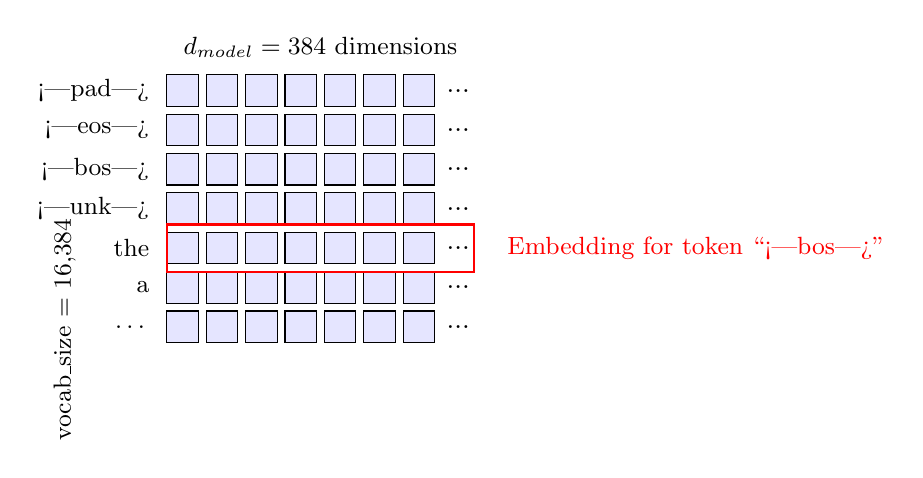
\begin{tikzpicture}[
    cell/.style={rectangle, draw, minimum width=0.4cm, minimum height=0.4cm, font=\tiny},
]
    % Draw matrix
    \foreach \y/\label in {0/<|pad|>, 1/<|eos|>, 2/<|bos|>, 3/<|unk|>, 4/the, 5/a, 6/\dots} {
        \node[left, font=\small] at (-0.3, -\y*0.5) {\label};
        \foreach \x in {0,...,7} {
            \ifnum\x=7
                \node at (\x*0.5, -\y*0.5) {...};
            \else
                \node[cell, fill=blue!10] at (\x*0.5, -\y*0.5) {};
            \fi
        }
    }

    % Labels
    \node[above, font=\small] at (1.75, 0.3) {$d_{\text{model}} = 384$ dimensions};
    \node[left, font=\small, rotate=90] at (-1.5, -1.5) {vocab\_size = 16,384};

    % Highlight one row
    \draw[thick, red] (-0.2, -2.3) rectangle (3.7, -1.7);
    \node[right, font=\small, red] at (4, -2) {Embedding for token ``<|bos|>''};
\end{tikzpicture}
\caption{The embedding table: each row is a token's learned vector representation}
\label{fig:embedding-table}
\end{figure}

\subsection{Memory Calculation}

The embedding table is often the largest part of a language model:

\begin{align*}
\text{Embedding parameters} &= \text{vocab\_size} \times d_{\text{model}} \\
&= 16,384 \times 384 \\
&= 6,291,456 \text{ parameters}
\end{align*}

At 4 bytes per float32 parameter:
\[
\text{Memory} = 6,291,456 \times 4 = 25.2 \text{ MB}
\]

\begin{keypoint}
For \TryLM, the embedding table contains $\sim$6.3 million parameters---more than half of the total $\sim$10.8 million parameters in the model!
\end{keypoint}

% -----------------------------------------------------------------------------
\section{Embedding Lookup}
% -----------------------------------------------------------------------------

The embedding operation is conceptually a \textbf{table lookup}:

\begin{lstlisting}[style=python]
import torch
import torch.nn as nn

# Create embedding table
embedding = nn.Embedding(vocab_size=16384, embedding_dim=384)

# Input: token IDs
token_ids = torch.tensor([1, 4521, 2378, 263])  # [BOS, Once, upon, a]

# Output: embeddings for each token
vectors = embedding(token_ids)
print(vectors.shape)  # torch.Size([4, 384])
\end{lstlisting}

\subsection{How It Works}

\texttt{nn.Embedding} uses the token ID as an index into the table:

\begin{lstlisting}[style=python]
# Conceptually equivalent to:
vectors = embedding.weight[token_ids]

# embedding.weight has shape [16384, 384]
# token_ids selects rows 1, 4521, 2378, 263
# Result has shape [4, 384]
\end{lstlisting}

\begin{figure}[H]
\centering
\begin{tikzpicture}[
    box/.style={rectangle, draw, minimum width=1.2cm, minimum height=0.6cm, font=\small},
    vec/.style={rectangle, draw, minimum width=2.5cm, minimum height=0.5cm, fill=green!20, font=\small},
    arrow/.style={-{Stealth[length=2mm]}, thick},
]
    % Input tokens
    \node at (-2, 2) {\textbf{Token IDs:}};
    \foreach \x/\t in {0/1, 1.3/4521, 2.6/2378, 3.9/263} {
        \node[box, fill=blue!10] at (\x, 2) {\t};
    }

    % Embedding table
    \node[rectangle, draw, minimum width=4cm, minimum height=2cm, fill=gray!10] (table) at (1.5, 0) {};
    \node[above] at (table.north) {Embedding Table};
    \node[font=\footnotesize] at (table.center) {\shape{16384, 384}};

    % Output vectors
    \node at (-2, -2) {\textbf{Embeddings:}};
    \foreach \x/\t in {0/$\mathbf{e}_1$, 1.3/$\mathbf{e}_{4521}$, 2.6/$\mathbf{e}_{2378}$, 3.9/$\mathbf{e}_{263}$} {
        \node[vec] at (\x, -2) {\t};
    }

    % Arrows
    \foreach \x in {0, 1.3, 2.6, 3.9} {
        \draw[arrow] (\x, 1.6) -- (\x, 1);
        \draw[arrow] (\x, -1) -- (\x, -1.6);
    }
\end{tikzpicture}
\caption{Embedding lookup: token IDs index into the embedding table to retrieve vectors}
\label{fig:embedding-lookup}
\end{figure}

\subsection{Batch Processing}

For a batch of sequences:

\begin{lstlisting}[style=python]
# Batch of sequences
batch = torch.tensor([
    [1, 4521, 2378, 263],   # Sequence 1
    [1, 487, 5831, 0],      # Sequence 2
])
# Shape: [2, 4] = [batch_size, seq_len]

vectors = embedding(batch)
# Shape: [2, 4, 384] = [batch_size, seq_len, d_model]
\end{lstlisting}

% -----------------------------------------------------------------------------
\section{Embeddings in TryLM}
% -----------------------------------------------------------------------------

Let's look at how \TryLM creates token embeddings:

\begin{lstlisting}[style=python, caption={Token embedding from model.py}]
class GPT(nn.Module):
    def __init__(self, config: ModelConfig) -> None:
        super().__init__()
        self.config = config

        # Token embeddings
        self.token_embedding = nn.Embedding(
            num_embeddings=config.vocab_size,  # 16384
            embedding_dim=config.d_model,      # 384
        )

        # ... rest of model
\end{lstlisting}

\subsection{In the Forward Pass}

\begin{lstlisting}[style=python, caption={Embedding lookup in forward pass}]
def forward(
    self,
    input_ids: Tensor,           # [batch, seq_len]
    attention_mask: Tensor | None = None,
    labels: Tensor | None = None,
) -> dict[str, Tensor]:

    # Convert token IDs to embeddings
    x = self.token_embedding(input_ids)  # [batch, seq_len, d_model]
    x = self.dropout(x)

    # ... pass through transformer blocks
\end{lstlisting}

% -----------------------------------------------------------------------------
\section{Weight Tying}
% -----------------------------------------------------------------------------

\TryLM uses a technique called \textbf{weight tying} (or \textbf{weight sharing}) between the input embeddings and the output projection.

\subsection{The Output Projection}

At the end of the model, we need to convert from hidden states back to vocabulary predictions:

\begin{lstlisting}[style=python]
# Hidden state: [batch, seq_len, d_model]
# We need: [batch, seq_len, vocab_size]

# Output projection (language model head)
self.lm_head = nn.Linear(
    in_features=config.d_model,      # 384
    out_features=config.vocab_size,  # 16384
    bias=False,
)
\end{lstlisting}

The \texttt{lm\_head} has shape \texttt{(vocab\_size, d\_model)}---exactly the same as the embedding table!

\subsection{Tying the Weights}

Instead of learning two separate matrices, we share them:

\begin{lstlisting}[style=python, caption={Weight tying from model.py}]
# Create embedding and output projection
self.token_embedding = nn.Embedding(config.vocab_size, config.d_model)
self.lm_head = nn.Linear(config.d_model, config.vocab_size, bias=False)

# Tie weights: lm_head uses the same matrix as token_embedding
self.lm_head.weight = self.token_embedding.weight
\end{lstlisting}

\begin{figure}[H]
\centering
\begin{tikzpicture}[
    box/.style={rectangle, draw, rounded corners, minimum width=3cm, minimum height=1cm, align=center},
    matrix/.style={rectangle, draw, minimum width=2cm, minimum height=1.5cm, fill=purple!20, align=center},
    arrow/.style={-{Stealth[length=2mm]}, thick},
]
    % Input path
    \node[box, fill=blue!10] (input) at (0, 2) {Token IDs\\$[B, S]$};
    \node[matrix] (emb) at (0, 0) {$W_e$\\$[V, D]$};
    \node[box, fill=green!10] (hidden) at (0, -2) {Hidden States\\$[B, S, D]$};

    % Output path
    \node[box, fill=orange!10] (logits) at (6, -2) {Logits\\$[B, S, V]$};
    \node[matrix] (head) at (6, 0) {$W_e^\top$\\$[D, V]$};
    \node[box, fill=green!10] (hidden2) at (6, 2) {Hidden States\\$[B, S, D]$};

    % Arrows
    \draw[arrow] (input) -- (emb) node[midway, right] {lookup};
    \draw[arrow] (emb) -- (hidden);
    \draw[arrow] (hidden2) -- (head) node[midway, right] {project};
    \draw[arrow] (head) -- (logits);

    % Tied weights connection
    \draw[thick, dashed, purple] (emb.east) -- (head.west) node[midway, above] {\textbf{Same weights!}};

    % Legend
    \node[font=\footnotesize] at (3, -3.5) {$B$ = batch, $S$ = sequence, $D$ = d\_model, $V$ = vocab\_size};
\end{tikzpicture}
\caption{Weight tying: the same matrix is used for input embeddings and output projection}
\label{fig:weight-tying}
\end{figure}

\subsection{Why Weight Tying?}

\begin{enumerate}
    \item \textbf{Fewer parameters}: We save $16,384 \times 384 = 6.3$M parameters
    \item \textbf{Semantic consistency}: The input and output use the same token representations
    \item \textbf{Better generalization}: Empirically improves performance on language modeling
\end{enumerate}

\begin{keypoint}
Weight tying connects the token-to-vector mapping (embedding) with the vector-to-token mapping (output projection). The model must use the same representations in both directions.
\end{keypoint}

% -----------------------------------------------------------------------------
\section{What Do Embeddings Learn?}
% -----------------------------------------------------------------------------

During training, the embedding vectors are updated to capture useful properties of tokens.

\subsection{Semantic Relationships}

After training, similar words have similar embeddings:

\begin{lstlisting}[style=python]
# After training, we can measure similarity
from torch.nn.functional import cosine_similarity

dog_emb = embedding(torch.tensor([dog_id]))
cat_emb = embedding(torch.tensor([cat_id]))
car_emb = embedding(torch.tensor([car_id]))

# Similar concepts are closer
cosine_similarity(dog_emb, cat_emb)  # High (e.g., 0.8)
cosine_similarity(dog_emb, car_emb)  # Lower (e.g., 0.3)
\end{lstlisting}

\subsection{Emergent Structure}

The embedding space develops structure through training:
\begin{itemize}
    \item Words that appear in similar contexts cluster together
    \item Grammatical categories (nouns, verbs) may form regions
    \item Related concepts maintain relative positions
\end{itemize}

\subsection{Visualization}

You can visualize embeddings using dimensionality reduction:

\begin{lstlisting}[style=python]
from sklearn.manifold import TSNE
import matplotlib.pyplot as plt

# Get embeddings for some words
word_ids = [tokenizer.encode(w)[1] for w in words]  # Skip BOS
word_embs = embedding.weight[word_ids].detach().numpy()

# Reduce to 2D
tsne = TSNE(n_components=2, random_state=42)
reduced = tsne.fit_transform(word_embs)

# Plot
plt.scatter(reduced[:, 0], reduced[:, 1])
for i, word in enumerate(words):
    plt.annotate(word, reduced[i])
\end{lstlisting}

% -----------------------------------------------------------------------------
\section{Embedding Initialization}
% -----------------------------------------------------------------------------

\TryLM initializes embeddings with small random values:

\begin{lstlisting}[style=python, caption={Weight initialization from model.py}]
def _init_weights(self, module: nn.Module) -> None:
    if isinstance(module, nn.Embedding):
        torch.nn.init.normal_(module.weight, mean=0.0, std=0.02)
\end{lstlisting}

\subsection{Why This Initialization?}

\begin{itemize}
    \item \textbf{Normal distribution}: Creates diverse initial representations
    \item \textbf{Small std (0.02)}: Prevents extreme initial values
    \item \textbf{Zero mean}: No bias toward positive or negative values
\end{itemize}

This is the standard initialization used in GPT-2/3 and most modern language models.

% -----------------------------------------------------------------------------
\section{Common Pitfalls}
% -----------------------------------------------------------------------------

\begin{pitfall}[title=Forgetting to Handle Unknown Tokens]
The embedding table has a fixed vocabulary. If you encounter an out-of-vocabulary token ID, you'll get an index error:

\begin{lstlisting}[style=python]
# vocab_size = 16384
embedding(torch.tensor([99999]))  # IndexError!
\end{lstlisting}

Always use the tokenizer's UNK token for unknown inputs.
\end{pitfall}

\begin{pitfall}[title=Mismatched Vocabulary Sizes]
The embedding vocab\_size must match the tokenizer:

\begin{lstlisting}[style=python]
# WRONG: mismatch causes errors
tokenizer = TryLMTokenizer.load(...)  # vocab_size=16384
model = GPT(ModelConfig(vocab_size=32000))  # Mismatch!

# CORRECT: must match
model = GPT(ModelConfig(vocab_size=tokenizer.vocab_size))
\end{lstlisting}
\end{pitfall}

% -----------------------------------------------------------------------------
\section{Exercises}
% -----------------------------------------------------------------------------

\begin{exercise}
\textbf{Calculate Embedding Memory}

For a model with vocab\_size=50,000 and d\_model=1024:
\begin{enumerate}
    \item How many parameters are in the embedding table?
    \item How much memory (in MB) for float32?
    \item With weight tying, how much do we save?
\end{enumerate}
\end{exercise}

\begin{exercise}
\textbf{Explore Embedding Dimensions}

Experiment with different embedding dimensions:
\begin{lstlisting}[style=python, numbers=none]
for d_model in [64, 128, 256, 384, 512]:
    emb = nn.Embedding(16384, d_model)
    params = emb.weight.numel()
    print(f"d_model={d_model}: {params:,} parameters")
\end{lstlisting}

How does model quality typically change with embedding dimension?
\end{exercise}

\begin{exercise}
\textbf{Verify Weight Tying}

After creating a model, verify that weights are tied:
\begin{lstlisting}[style=python, numbers=none]
from trylm.model import GPT
from trylm.config import ModelConfig

model = GPT(ModelConfig())

# Check if weights are the same object
print(model.token_embedding.weight is model.lm_head.weight)  # True?

# Check if values are identical
print(torch.equal(model.token_embedding.weight,
                  model.lm_head.weight))  # True?
\end{lstlisting}
\end{exercise}

% -----------------------------------------------------------------------------
\section{Summary}
% -----------------------------------------------------------------------------

\begin{summary}
    \item \textbf{Embeddings} convert discrete token IDs to continuous vectors
    \item The \textbf{embedding table} has shape \texttt{(vocab\_size, d\_model)}
    \item \texttt{nn.Embedding} performs efficient \textbf{table lookup}
    \item \textbf{Weight tying} shares parameters between embedding and output projection
    \item Embeddings are \textbf{learned} during training to capture token semantics
    \item For \TryLM, embeddings account for $\sim$6M of $\sim$11M total parameters
\end{summary}

With token embeddings, we've converted token sequences into continuous representations. In the next chapter, we'll see how the model processes these embeddings using self-attention---the core mechanism that allows tokens to ``communicate'' with each other.
